\chapter{Mikroskopische Thermodynamik}
\label{kap_mikroskopische-thermodynamik}




In diesem Kapitel betrachten wir einzelne Atome, Molek"ule oder einfach
kleinste Teilchen -- jedoch versuchen war gar nicht erst, f"ur die
gro"sen Mengen an Teilchen exakte Bewegungsgleichunge zu l"osen, sondern
verwenden die Aussagen aus der Thermodynamik (Kap
\ref{kap_thermodynamik}), die wir aus Beobachtungen des Makrozustandes
gewonnen haben, und untersuchen damit das Verhalten der kleinsten
Teilchen.

Wir verlassen uns also auf \emph{statistische} Ans"atze, die uns zwar
keine exakten Aussagen erm"oglichen, daf"ur aber eine Aussage, die
f"ur ein Teilchen \emph{im Allgemeinen} gilt. Eine wohldefinierte,
konstante (makroskopische) Zustandsgr"o"se ist auf der mikroskopischen
Scala unter Umst"anden starken Schwankungen unterworfen -- so als
w"urden wir unsere Messergebnisse jetzt unter dem Mikroskop
betrachten.

Wie im \textsc{Feynmann}'schen Experiment der \textbf{Molekularen
  Ratsche} kann es dabei zu eigentlich verwirrenden Ergebnissen kommen
-- die sich aber doch wieder logisch "uber bekannte physikalische
Probleme erkl"aren lassen.






\section{\textsc{Stokes-Einstein}-Relationen}
\label{kap_stokes-einstein-relationen}

Wir betrachten $N$ \index{Kolloid}Kolloide\footnote{Kleine
  Teilchen ($d \approx 1 \operatorname{\mu m}$) die jedoch noch
  \emph{weit gr"o"ser} sind, als die Teilchen der L"osung. Eine
  \emph{kolloidale L"osung} kann bspw. ein klares L"osungsmittel sein,
  in dem so viele Kolloide das Licht streuen, dass die Fl"ussigkeit
  eine milchige Tr"ubung erh"alt.}, die in einem Fl"ussigkeitsvolumen
$V$ \index{Suspension}suspendiert\footnote{Ein Feststoff ist in einer
  Fl"ussigkeit fein verteilt, aber immer noch im festen
  Aggregatszustand.} sind und definieren die \textbf{Teilchendichte}:
\begin{equation}
   \label{eqn_def_teilchendichte}
   n_K = \frac{N}{V} = \frac{p}{K_B T}
\end{equation}
Sei nun $n_K$ hinreichend klein -- also wenige dieser Kolloide
"`gel"ost"', so kann man die Kolloide als Ideales Gas behandeln (und
die Fl"ussigkeit als Vakuum zwischen den "`Gasteilchen"').


\subsection{Betrachtung als Kr"aftegleichgewicht}
\label{kap_betrachtung-als-kraftegleichgewicht}


Die "`Gasteilchen"' respektive Kolloide erzeugen den Druck
\begin{equation}
   \label{eq:13}
   p = n_K \cdot K_B \cdot T
\end{equation}
%
%\abs
Auf die Kolloide wirkt noch eine weiter Kraft $F$ --
bspw. \emph{Graviatation}, ein \emph{elektrisches Feld} etc. Im
Thermischen \emph{Gleichgewicht} gilt:
$$
 \sum_i F_i = 0
$$
und so f"ur die \emph{\index{Kraftdichte}Kraftdichten} 
\begin{Def}
   [Kraftdichte $\vec f$] Die Kraftdichte $\vec f$ ist als "`Kraft pro
   Volumen"' so definiert, dass 
   \begin{equation}
      \label{eq:210}
\diff \vec F = \vec f \diff V ~ \text{ oder } ~ \vec F = \int_V \vec f \diff V
   \end{equation}
 ist.
\end{Def}
Die Kraftdichte ergibt sich aus dem Druck durch
\begin{equation}
   \label{eq:208}
   \vec f = \vec f(\vec r) = - \vec \nabla p(\vec r)
\end{equation}
Wenn die Kr"afte auf alle $N$ Teilchen der Teilchendichte $n = \frac{N}{V}$ gleich
wirken  und auf jedes Teilchen  die Kraft $\vec F$ wirkt, so folgt f"ur die
Kraftdichte und weil insgesamt die Kraft $N\, \vec F$ wirkt:
\begin{equation*}
\vec f = \frac{N \, \vec F}{V} = \vec F \cdot n
\end{equation*}
Damit und der Definition aus Gl. \eqref{eq:210} folgt so:

\begin{equation}
   \label{eq:14}
   n_K(\vec r) \cdot \vec F + \Vec \nabla p(\vec r) = 0
\end{equation}
mit Gl. \eqref{eq:13} folgt
\begin{equation}
   \label{eq:15}
   \frac{p(\vec r)}{K_B T} \cdot \vec F + \vec \nabla p(\vec r) = 0
\end{equation}
Dies ist eine (partielle) Differentialgleichung mit der L"osung
\begin{equation}
   \label{eq:16}
   p(\vec r) = \underbrace{\exp \left ( - \frac{\vec F \cdot \vec
          r}{K_B T} \right )}_\text{ \textsc{Boltzmann}-Faktor } ~ \sim
   ~ n_K(\vec r)
\end{equation}
Die Proportionalit"at zu $n_K$ ergibt sich aus Gl. \eqref{eq:13}. Dies
ist eine
\emph{\textsc{\index{Boltzmann-Verteilung}Boltzmann}-Verteilung}!

\abs
Nun k"onnen wir als Spezialfall die \textbf{Gravitation} als Kraft
verwenden mit $\vec F = m \cdot \vec g$:
\begin{equation}
   \label{eqn_barometrische-hoehenformel-thermo}
   n_K(h) \sim 
\exp \left ( - \frac{mg \cdot h}{K_B T} \right )
\end{equation}
und erhalten die \textbf{\index{Barometrische H"ohenformel}Barometrische
H"ohengleichung}; die Kolloide
in der L"osung verhalten sich also wie die Luft in der Atmosph"are.




\subsection{Betrachtung mit Teilchenstrom}
\label{kap_betrachtung-mit-teilchenstrom}

Der Gleichgewichtszustand des Systems ist Ergebnis zweier
gegenl"aufiger Teilchenstr"ome.

\begin{Def}
   [\index{Teilchenstrom}Teilchenstrom $\vec j$]
gibt an, wie sich die Teilchen\emph{dichte} ausbreitet (nicht
ein einzelnes Teilchen).
Es gilt
\begin{equation}
   \label{eqn_def_teilchenstrom}
   \vec j = n_K(\vec r) \cdot \vec v ( \vec r )
\end{equation}
\end{Def}

Bei uns laufen gegeneinander
\begin{enumerate}
\item \index{Diffusionsstrom}Diffusionsstrom\\Teilchen str"omen nach oben, weil oben im Gef"a"s
   die Dichte kleiner ist. Die Diffusion l"auft entgegen des
   Gradienten\footnote{weil der Gradient ja in die Richtung der
     \emph{gr"o"sten} "Anderung zeigt, also dorthin, wo die Dichte weiter
   zunimmt}:
   \begin{equation}
      \label{eqn_diffusionsstrom}
      \vec j_\text{dif} =  - D \cdot  \nabla n_K(h)
   \end{equation}
   Dabei ist $D$ der
   \emph{\index{Diffusionskoeffizient}Diffusionskoeffizient} (mit $[D]
   = \frac{m^2}{s}$).

   Nur mit der Diffusion w"urden die Teilchen sich lediglich
   gleichverteilen.

\item Driftstrom\\Durch die Schwerkraft str"omen Teilchen nach
   unten. Mit der \textsc{Stokes}-Reibung 
$$
\vec F = 6 \pi \eta r \vec v
$$
mit der Viskosit"at $\eta$ und dem Teilchenradius $r$ ergibt sich (im
Gleichgewicht):
\begin{equation}
   \label{eqn_driftstrom}
   \vec j_\text{drift} = n_K \cdot \vec v = n_K \cdot \frac{\vec
     F}{6\pi\eta r}
\end{equation}
\end{enumerate}
Im Gleichgewicht gilt nun:
$$
\vec j_\text{dif} + \vec j_\text{drift} = 0
$$
und mit Gl. \eqref{eqn_diffusionsstrom} und \eqref{eqn_driftstrom}
gilt:
\begin{equation}
   \label{eq:10}
 D \cdot  \nabla n_K(h) =   n_K \cdot \frac{\vec
     F}{6\pi\eta r}
\end{equation}
Setzt man auf der linken Seite f"ur $n_K(h)$
Gl. \eqref{eqn_barometrische-hoehenformel-thermo} ein gilt mit 
$$
\nabla n_K(\vec h) = \nabla \exp \left ( - \frac{m\, \vec g \cdot \vec
     h}{K_B T} \right ) = - \frac{m\, \vec g}{K_B T} \cdot \exp \left ( -
   \frac{m\vec g \cdot \vec h}{K_B T} \right ) = - \frac{\vec F_g}{K_B
  T} \cdot n_K(\vec h)
$$
und da $\vec F = -\vec F_g$ gilt f"ur Gl. \eqref{eq:10}:
\begin{equation*}
   \label{eq:17}
   D \cdot \frac{\vec F}{K_B T} \cdot n_K(h) =  n_K \cdot \frac{\vec
     F}{6\pi\eta r}
\end{equation*}
und so aufgel"ost nach $D$ ergibt sich die
\textbf{\textsc{Stokes-Einstein}-Relation}:
\begin{equation}
   \label{eqn_stokes-einstein-relation}
   \boxed{   
     D = \frac{K_B T}{6\pi\eta r} 
   }
\end{equation}


An dieser ist interessant, dass sie -- ganz im Geiste der
Mikroskopischen Thermodynamik -- die makroskopische Gr"o"se $D$ in
Zusammanhang bringt mit den atomaren Gr"o"sen $\eta$ und $r$.






\subsection{Mittlere Freie Wegl"ange}
\label{kap_mittlere-freie-weglange}

\begin{Def}
   [\index{Mittlere Freie Wegl"ange}Mittlere Freie Wegl"ange $\lambda$
   oder $\ell$] L"ange $\lambda$, wie weit sich ein Teilchen bewegn
   kann, ohne mit einem anderen zu kollidieren.
\end{Def}

\begin{Wichtig}
   Der mittlere Teilchenabstand $\bar a$ ist verschieden von der
   mittleren freien Wegl"ange $\lambda$.
\end{Wichtig}

Wir unterteilen das Volumen $V$, welches $N$ Teilchen enth"alt, nun in
$N$ W"urfel mit der Kantenl"ange $a$; und
% $$
% V = N \cdot a^3
% $$
mit \eqref{eqn_def_teilchendichte} folgt
\begin{equation}
\label{eq:18}
   V = Na^3 = \frac{N}{n_K} ~ \Rightarrow ~ \frac{1}{n_K} = a^3
~ \Rightarrow ~
\sqrt[3]{\frac{1}{n_K}} = n_K^{-\frac{1}{3}}= a 
\end{equation}
Es ist nun $a = \bar a \neq \lambda$: Denken wir uns die Gasteilchen
gleichverteilt -- mit Verteilung $n_K$ -- so hat jedes f"ur sich einen
eigenen kleinen W"urfel mit Kantenl"ange $a$. Denken wir nun, dass
jedes Teilchen sich nur in seinem W"urfel bewegt, so haben sie im
Mittel den Abstand $\bar a$ voneinander.

\bigskip Wir betrachten nun einen Quader mit L"ange $\diff x$ und
Seitenfl"ache $A$, in dem sich $N$ Teilchen (mit Dichte $n_K$) befinden
und sich bewegen. Von au"sen fliegt ein weiteres Teilchen auf $A$
zu. Man projeziert nun die Teilchen \emph{im} Quader parallel zur
Bewegung $\vec v$ des anfliegenden Teilchens auf die Fl"ache $A$. Ein
Teilchen mit Radius $r$ nimmt hier die Fl"ache 
\begin{equation}
   \label{eq:18b} 
   \sigma = \pi r^2
\end{equation}
ein -- die $N$ Teilchen logischerweise die Fl"ache $N \cdot \sigma$.

Die Wahrscheinlichkeit, dass das anfliegende Teilchen in der Zeit
$\diff t$ ein Teilchen im Quader erwischt ist
\begin{equation}
   \label{eq:19}
   \frac{A_\text{Teilchen}}{A_\text{Fl"ache insgesamt}} =
   \frac{\overbrace{n \cdot \overbrace{A \cdot \diff x}^V}^N \cdot
     \sigma}{A}
= n \cdot \sigma \cdot \diff x
\end{equation}
Aufgrund von Kollisionen nimmt die Zahl $j$ von Teilchen in $V$, die sich in
Richtung $\vec v$ bewegen (und so mit dem anfliegenden sto"sen), immer
weiter ab, je weiter man sich in $V$ hereinbewegt:
\begin{equation}
   \label{eqn_differenz-c0}
   j(x + \diff x) = j(x) - j(x) \cdot n \sigma \diff x
\end{equation}
(wir subtrahieren auf dem Weg nach $x$ von den sto"sbereiten Teilchen
$j$ die Teilchen, mit denen das anfliegende zusammenprallen wird ($j
\cdot n\sigma \diff x$, weil nach \eqref{eq:19} dies angibt, mit wie
vielen Teilchen aller
\emph{Wahrscheinlichkeit} nach das anfliegende sto"sen wird). 

Subtrahiren wir in \eqref{eqn_differenz-c0} $j(x)$ und teilen durch $\diff x$, so
haben wir eine Differentialgleichung. Eine L"osung ist
\begin{equation}
   \label{eqn_differenz-c1}
   j(x) = j_0 \cdot \exp ( - n \sigma x )
\end{equation}
Wir interpretieren das Ergebnis jetzt als \emph{Verteilung}: Je gr"o"ser
der Abstand $x$ wird, desto geringer ist die Wahrscheinlichkeit, dass
das Teilchen noch mit einem anderen st"o"st -- aber daf"ur ist die
Wahrscheinlichkeit, dass das Teilchen schon sehr fr"uh st"o"st,
au"serordentlich hoch, d.h. nur wenige Teilchen kommen "uberhaupt in die
N"ahe der gro"sen $x$. \eqref{eqn_differenz-c1} ist also die Verteilung der
Teilchen mit denen dein anfliegendes sto"sen kann, wobei $x$ dann
logischerweise f"ur die Strecke \emph{vor} dem Sto"s -- also die freie
Wegl"ange $\lambda$ -- steht.

Um jetzt noch die \emph{mittlere} freie Wegl"ange zu bestimmen,
verwenden wir eine Eigenschaft der $e$-Funktion: Das Mittel liegt bei
$y = \frac{1}{e}$; in unserem Fall also bei $\frac{1}{e} \cdot
j_0$. Mit $x = \lambda$ gilt:
\begin{equation}
   \label{eqn_differenz-c2}
   \boxed{
\lambda = \frac{1}{n \cdot \sigma}
}
\end{equation}



\subsection{Alternative Herleitung und Wirkungsquerschnitt $(\bigstar)$}
\label{kap_altern-herl-und-wirk-bigst}


In der vorhergehenden -- etwas weitschweifigen -- Herleitung haben wir
quasi nebenher bestimmt, mit welcher Wahrscheinlichkeit ein Teilchen,
welches sich um $x$ bewegt, st"o"st (Gl. \eqref{eqn_differenz-c1}).

Eine wesentlich \textbf{einfachere Herleitung} f"ur die mittlere freie
Wegl"ange $\lambda$ geht folgenderma"sen vor: Ein Teilchen habe wieder
die (effektive) Fl"ache $\sigma$ zu seiner
Bewegungsrichtung\footnote{Also die Projektion parallel der
  Bewegungsrichtung auf eine Fl"ache senkrecht zur Bewegungsrichtung
  ist $\sigma$.}. Wenn dieses Teilchen sich im Volumen $V$ mit
insgesamt $N$ Teilchen bewegt, so wird es \emph{im Mittel} (so ist ja
$\lambda$ definiert) die Strecke $\lambda$ zur"ucklegen k"onnen, ohne
gegen ein anderes Teilchen zu sto"sen. Dabei "uberstreicht es das
Volumen
\begin{equation*}
   V_{\lambda} = \sigma \cdot \lambda
\end{equation*}
Nun hat jedes Teilchen das selbe Volumen zur Verf"ugung -- also bei $N$
Teilchen folgt so -- wesentlich schneller --
\begin{equation}
   \label{eq:204}
   V_\lambda = \frac{V}{N} = \frac{1}{n} \equiv \sigma \cdot \lambda
   \text{ oder } ~ \lambda = \frac{1}{n \cdot \sigma}
\end{equation}


\abs Der \emph{Hintergrund} ist, dass in dieser kurzen Herleitung
$\sigma$ einfach als Querschnittsf"ache interpretiert wurde, in der in
der ersten Herleitung dagegen als
\textbf{\index{Wirkungsquerschnitt}Wirkungsquerschnitt}. Dieser ist
definiert als Ma"s f"ur die Wahrscheinlichkeit, dass ein bestimmter
Wechselwirkungsprozess (in unserem Falle ein Sto"s) zwischen Teilchen
eines Teilchenstrahls und einem Streuzentrum (hier die anderen
Teilchen) eintritt. Dieses Ma"s ist der Quotient aus gestreuten
Teilchen zum Teilchenfluss:
\begin{equation*}
   \sigma = \frac{\text{Gestreute Teilchen pro
       Zeit}}{\text{Anfliegende Teilchen pro Zeit und Fl"ache}}
\end{equation*}
und hat damit die \emph{Dimension} einer Fl"ache.

Alternativ kann man die anfliegenden Teilchen auch als Punktf"ormig
interpretieren. Dann stellt $\sigma$ eine Fl"ache auf dem Ziel
senkrecht zur Bewegungsrichtung des anfliegenden Teilchens dar, wobei
die Wechselwirkung stattfindet, wenn das Punktteilchen in $\sigma$
trifft und ausbleibt, wenn es an $\sigma$ vorbeigeht. Damit ist
$\sigma$ auch ein Ma"s f"ur die "`St"arke"' der Wechselwirkung. 

Die Wahrscheinlichkeit $w$ f"ur eine Wechselwirkung ergibt sich bei
einer Targetfl"ache von $A_T$ und $N_T$ Targetteilchen zu
\begin{equation*}
   w = \frac{\sigma \, N_T}{A_T} = \frac{N_W}{N} \text{ und damit } 
 \frac{\sigma}{A_T} = \frac{\frac{N_W}{N}}{N_T} = \frac{w}{N_T}
\end{equation*}
Hier bezeichnet $N_W$ die (angeflogenen) Teilchen, die gewechselwirkt
haben und $N$ die insgesamt angeflogenen Teilchen. 

Betrachten wir nun ein (d"unnes) Teilchenvolumen $V_T = A_T \cdot \diff
x$, so ist die Wahrscheinlichkeit f"ur einen Sto"s hier
\begin{equation*}
   w = \frac{N_W}{N} = \frac{\sigma \, N_T \cdot \diff x}{A_T \cdot \diff x}
=
\frac{\sigma \, \diff x \cdot N_T}{V_T} = \sigma \, n_T \, \diff x
\end{equation*}
wobei wir mit $n_T$ die \emph{Teilchendichte} der Zielteilchen
bezeichnen.  Bei dem Durchfliegen von $\diff x$ "`verliert"' man also
$w \cdot N$ Teilchen und hat so (wenn $N_0$ die anf"angliche
Teilchezahl im Teilchenstrahl war) $N_0 - N_W$ Teilchen "ubrig; damit
ist $N_W = - \Delta N$. Bei infinitissimaler Betrachtung f"uhrt das zu
\begin{equation*}
   - \diff N = N \cdot w = N \cdot \sigma n_T \, \diff x
\end{equation*}
und die L"osung dieser DGL (durch $N$ teilen und aufintegrieren) ist
\begin{equation*}
   N = N(x) = N_0 \E^{- \sigma n_T \, x} 
\end{equation*}
Wir betrachten nun, wann der Strahl auf $\frac{1}{\E}$ seiner
urpsr"unglichen Indensit"at abgesunken ist\footnote{Diese Betrachtung
  ist "ublich: Bei radioaktivem Zerfall betrachtet man die Zeit $\tau$,
zu der $\frac{1}{\E}$ des Urspr"unglichen Materials "ubrig ist, anstatt
der \emph{Halbwertszeit} $T_{1/2}$.}, also wenn $N(x) = \frac{1}{\E}\, N_0$.
Ein einfacher Koeffizientenvergleich liefert dann
\begin{equation*}
   \sigma n_T \, x = 1 ~  \text{ oder }  ~ \lambda = \frac{1}{n_T \, \sigma}
\end{equation*}
und danach definiert man die \emph{mittlere Freie Wegl"ange} $x \equiv \lambda$,
die diese Gleichung l"ost.

% Bewegen sich die Teilchen also $L$ in das Target hinein, sind $N(L)$
% Teilchen im Teilchenstrom "ubrig. F"ur $\sigma$ gilt dann:
% \begin{equation*}
%    \sigma = \frac{1}{n \, L} \cdot \ln \frac{N_0}{N(L)}
% \end{equation*}












\subsection{Exkurs: \textsc{Boltzmann}-Faktor und Thermische Energie}
\label{kap_exkurs:bolzmann-faktorn-und-thermische-energie}

In Gl. \eqref{eqn_barometrische-hoehenformel-thermo} haben wir eine
\textsc{Boltzmann}-Verteilung gesehen, die in ihrem Argument von
potentieller Energie ($mg$ bei der Schwerkraft) und der Thermischen
Energie ($T$) abh"angt. 

"Uber diesen Zusammenhang k"onnen wir eine Verteilung $n(E)$ definieren,
wobei $n$ der Besetzungswahrscheinlichkeit f"ur das Energieniveau $E$
entspricht\footnote{in $E$ stecken verschiedene Energieformen -- die
  thermische und dann noch potentielle oder kinetische oder ...}:
\begin{equation}
   \label{eqn_bolzmann-verteilung}
   n(E) = n(E = 0) \cdot \exp \left ( - \frac{E}{K_B \cdot T} \right )
\end{equation}
\begin{Wichtig}
   Die Boltzmann-Verteilung gilt immer nur im Gleichgewicht!
\end{Wichtig}



%\paragraph{Beispiel: Energiezust"ande im Atom}
%\label{kap_beispiel:-im-atom}


\begin{Beispiel}

   \emph{Energiezust"ande im Atom:} Hier gibt $n$ die
   Wahrscheinlichkeit daf"ur an, dass ein bestimmter Zustand besetzt
   ist. f"ur zwei Zust"ande $E_1$ und $E_2$ gilt:
\begin{equation*}
   n(E_i) = n_0 \cdot \exp \left ( - \frac{E_i}{K_B \cdot T} \right ) ~
      \Rightarrow ~ \frac{n(E_1)}{n(E_2)} = 
\exp \left ( - \frac{\Delta E}{K_B \cdot T} \right )
\end{equation*}
Nehmen wir nun an, $\Delta E > 0$ (also $E_2$
h"oherenergetisch\footnote{da $\Delta E = E_2 - E_1$.}), so ist
$\frac{\Delta E}{K_BT} \geq 0$ und damit $\exp \left ( - \frac{\Delta
     E}{K_B \cdot T} \right ) < 1$. D.h. die Wahrscheinlichkeit, dass
Zustand $E_2$ besetzt ist, ist niedriger, da Energetisch ung"unstiger.
\end{Beispiel}

















\section{Entropie des idealen Gases}
\label{kap_entropie-des-idealen-gases}


Wir hatten in Gl. \eqref{eqn_def_entropie} schon eine Definition der
\index{Entropie}Entropie:
$$
\diff S = \frac{\diff Q}{T}
$$
Hier wollen wir aber noch eine zweite kennenlernen und die Entropie
zun"achst naiv als \emph{Ma"s der Unordnung} eines Systems betrachten.

Dazu definieren wir $\Omega$ als \emph{Anzahl der m"oglichen
  Zust"ande}, die ein System einnehmen kann.\footnote{Etwas genauer:
  $\Omega$ gibt ein \emph{Volumen} im
  \emph{\index{Phasenraum}Phasenraum} an. Der Phasenraum ist ein
  Vektorraum, der durch die Ver"anderlichen eines Systems aufgespannt
  wird, welche das System vollst"andig characterisieren. Ein Punkt in
  diesem Raum entspricht dann einer Kombination dieser
  Ver"anderlichen: Einem \emph{Zustand}. Bspw. verwenden wir in
  Kap. \ref{kap_zustandsflachen-des-idealen-gases} auch eine Art
  Phasenraum; wenn wir im $\mathbb R^3$
  (s. Abb. \ref{abb_ideale-gasgleichung}) eine Fl"ache darstellen,
  entspricht diese Fl"ache einer Einschr"ankung des dreidimensionalen
  Phasenraums auf zwei Dimensionen.

  Je gr"o"ser das Volumen dieses Raums ist, desto mehr Punkte enth"alt er
  und folglich ist so die Anzahl der m"oglichen Kombinationen gr"o"ser.}
Dann gilt f"ur die \textbf{Entropie} n"amlich:
\begin{equation}
   \label{eqn_def_entropie_zustaende}
   S = K_B \cdot \ln \Omega
\end{equation}
Da die Entropie eines Systems stets bestrebt ist, zu wachsen
(s. Kap. \ref{kap_zweiter-hauptsatz}) k"onnte man nun annehmen, dass
wenn die Entropie steigt und folglich auch $\Omega$ steigen muss, das
System zwangsl"aufig unordentlicher wird; dem ist aber nicht so.

\begin{Wichtig}
   Die Entropieerh"ohung eines Systems kann auch Ordnung erzeugen!
\end{Wichtig}

\begin{Def}
   [\index{Entropische Kr"afte}Entropische Kr"afte] Kr"afte, die nur
   auftreten, damit die Entropie maximiert wird.
\end{Def}


\subsection{Kristallisation von harten Kugeln}
\label{kap_kristallisation-von-harten-kugeln}

Harte Kugeln haben ein rein repulsives Potential, welches nur auf
n"achste N"ahe (eig. bei Kontakt)  wirkt:
\begin{equation}
   \label{eqn_potential_hate_kugeln}
   V(d) \sim \delta(d)
\end{equation}
Wobei $\delta$ die \textsc{Dirac}'sche Deltafunktion ist und $d$ der
Abstand der beiden Kugeloberfl"achen voneinander. Die Kugeln sto"sen
sich also genau dann ab, wenn sie sich ber"uhren.

Die Energie eines Systems solcher Teilchen ist unabh"angig von der Lage
der Teilchen zueinander, weil die Kugeln ja keine Kr"afte aufeinander
aus"uben. Da somit die Innere Energie $U = const$ ist, k"onnen wir sie
\emph{definieren} als 
$$
 U = 0
$$
und mit Gl. \eqref{eqn_freie-energie} k"onnen wir folgern:
\begin{equation}
   \label{eqn_differenz-c3}
   \mathcal F = - T \cdot S
\end{equation}
ein solches System bezeichnen wir als \emph{rein entropisch}:
\begin{Def}
   [\index{Rein entropisches System}Rein entropisches System]
Das Verhalten eines Systems wird alleine durch dessen Entropie bestimmt.
\end{Def}

Da wir eine \emph{spontane} Kristallisation unserer Kugeln wollen,
muss nach Kap. \ref{kap_zweiter-hauptsatz} gelten: 
$$
\diff S > 0
$$
D.h. f"ur die Freie Energie $\mathcal F$ in fl"ussigem bzw. kristallinem
Zustand muss gelten:
$$
\mathcal F_\text{fl} > \mathcal F_\text{kr}
$$

\bigskip
In einem normalen atomaren System sieht das Potential
der Wechselwirkungskr"afte aus wie in
Abb. \ref{abb_kristallpotential}. Bei diesem ist die Kraft bei gro"sen
Abst"anden noch attraktiv (im Schaubild bis dieses seinen Tiefpunkt
erreicht). Hier wirken die
\textsc{Van-Der-Waals}-Wechselwirkungen. Danach wird die Kraft
repulsiv, weil sich die gleich geladenen Atome absto"sen. Die
Kristallation eines Stoffes kommt dann daher, dass sich die Teilchen
so nahe kommen, dass sie den Tiefpunkt des Potentials erreicht haben
und hier in einer station"aren -- stabilen -- Entfernung voneinander
liegen und sich so nicht weg bewegen lassen. Der Kristall ist
entstanden und stabil.
\begin{figure}
   \centering
   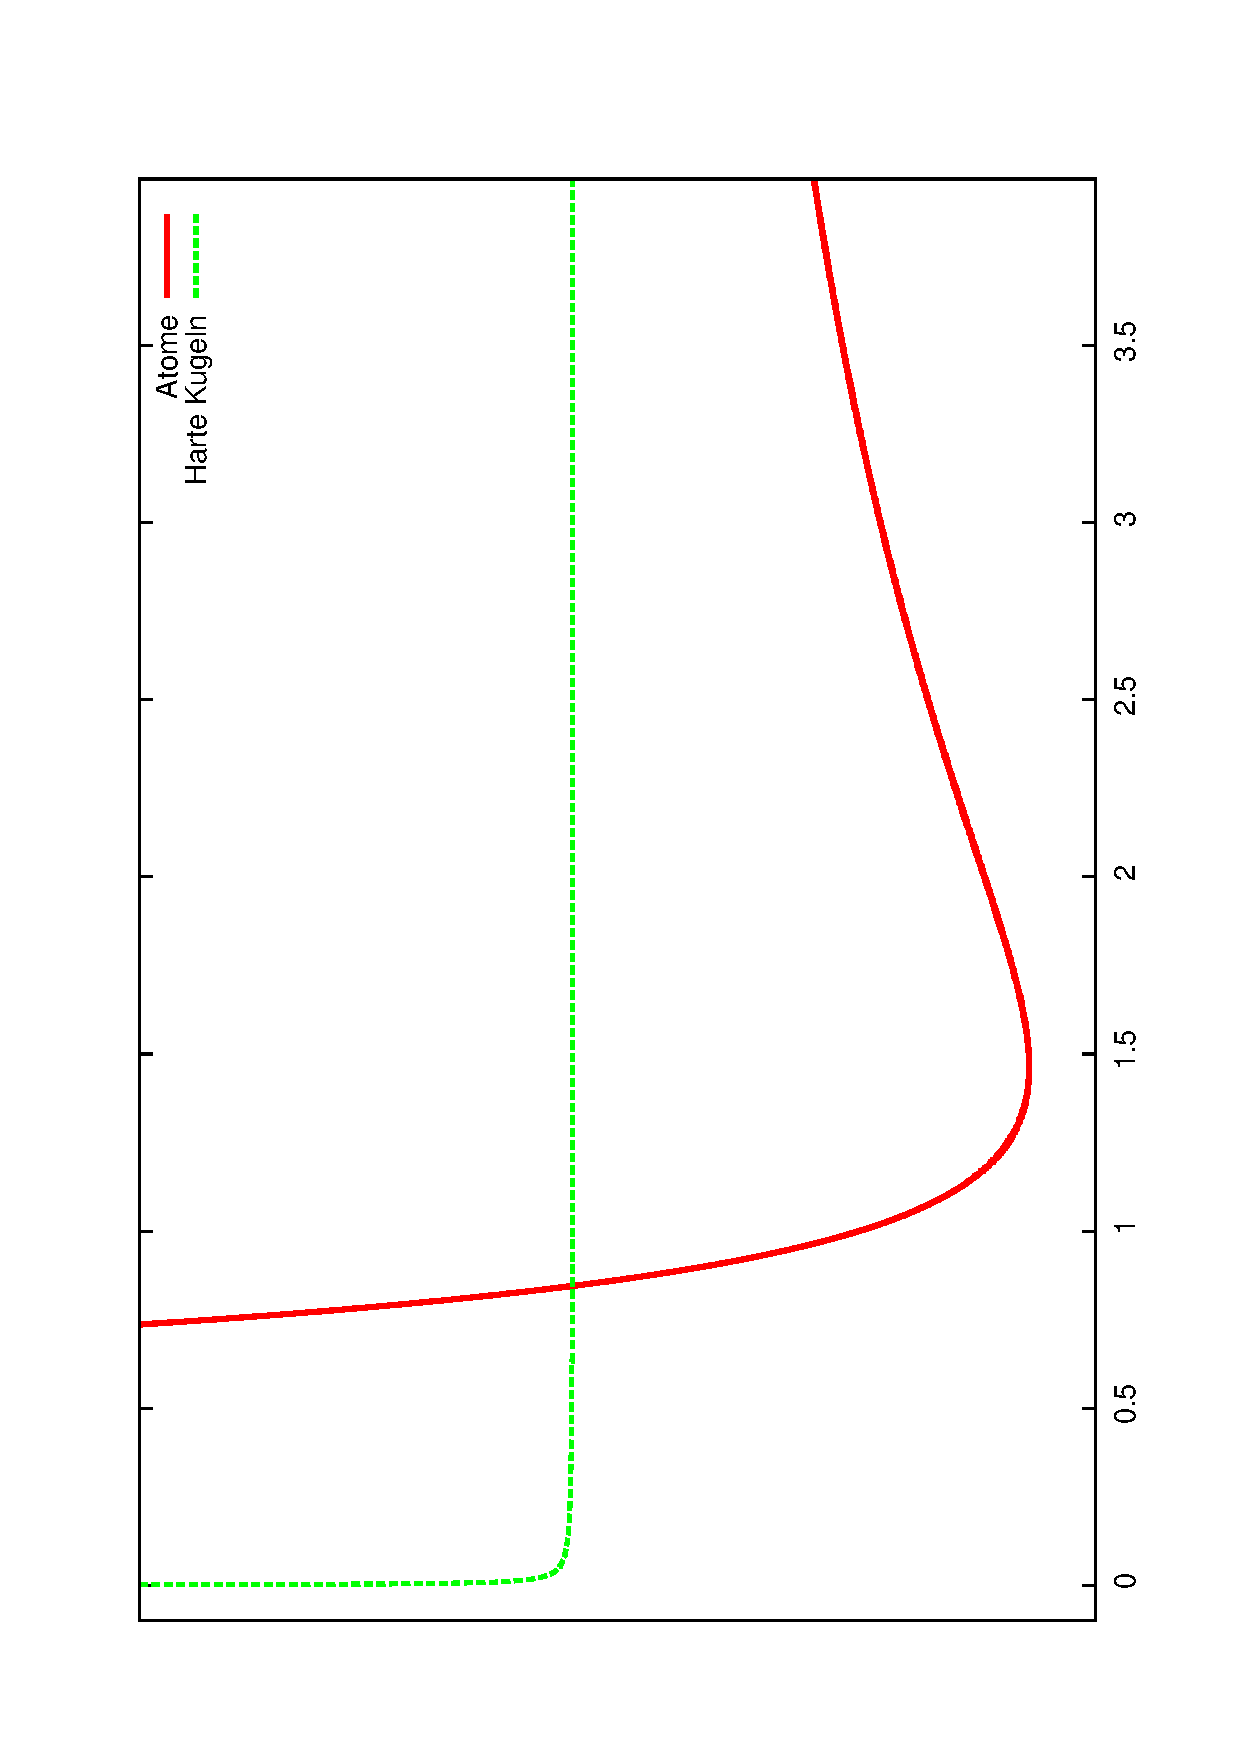
\includegraphics[width=0.7\textwidth,angle=-90]{bilder/kristallpot2}
   \caption[Potentiale: Atomar, Harte Kugeln]{Potential zwischen den
     Atomen bei einem nat"urlichen Kristall und bei Harten Kugeln;
     links im Schaubild sind sich die Atome bzw. Kugeln n"aher.}
   \label{abb_kristallpotential}
\end{figure}


Nun ist es im Falle der Harten Kugeln aber so, dass wir kein
solches Potential haben! Wir k"onnen bei den Harten Kugeln die
Kristallisation nicht mit einem solchen Energieminimum erkl"aren, weil
wir keine attraktiven Wechselwirkungen vorweisen k"onnen.

Stattdessen untersuchen wir zwei verschiedene Arten der Entropie:
\begin{enumerate}
\item Konfigurationsentropie $S_K$\\
   H"angt ab von der Anzahl verschiedener M"oglichkeiten, wie man die
   Harten Kugeln in einem gegebenen Volumen anordnen kann. Die Zahl
   der M"oglichkeiten, wie man Kugeln zu einem Kristall anordnen kann
   ist logischerweise \emph{kleiner}, als eine Fl"ussigkeit zu bilden:
$$
S_{K, \text{fl}} \gg S_{K, \text{kr}}
$$
\item Entropie des freien Volumens $S_V$\\
   Bei gegebener Konfiguration kann sich jedes Teilchen ein wenig um
   seine Ruhelage bewegen. Je nach dem, wie viel Volumen das Teilchen
   um seine Ruhelage herum hat, kann es sich weiter bewegen.
\end{enumerate}

Wir untersuchen nun $S_V$ f"ur verschiedene Kugelpackungen und finden
heraus, dass wenn man die Kugeln kristallf"ormig anordnet, die
einzelnen Teilchen mehr Platz um sich haben: Bei einer ungeordneten
Kugelpackung kann man maximal $64\%$ des Volumens mit Kugeln ausf"ullen
-- bei geordneten Kugeln sind es bis zu $74\%$. \footnote{Ab einer
  Packungsdichte von $49\%$ tr"agt $S_V$ schon zu einer Erh"ohung von
  $S$ bei und sorgt so daf"ur, dass sich das System spontan anordnet.}

Da also im Kristall mehr Kugeln in das selbe Volumen gehen, brauchen
gleich viele Kuglen im Kristall weniger Platz und so kann dieser
Unterschied an Platz als Bewegungsfreiraum herhalten, der $S_V$
erh"oht.

Da
$$
S = S_K + S_V
$$
gilt, ist die Entropie im Geordneten System gr"o"ser -- und nach
Gl. \eqref{eqn_differenz-c3} ist hier die Freie Energie \emph{kleiner}.

\begin{Wichtig}
   Die Harten Kugeln erreichen ihr Energieminumum also, wenn sie
   kristallisieren.
\end{Wichtig}








\subsection{Quantitative Beschreibung entropischer Kr"afte}
\label{kap_quantitative-beschreibung-entropischer-krafte}


Wir betrachten ein System mit einer gro"sen Harten Kugel (Rad. $R$) und um sie
herum $N$ kleine Kugeln (Rad. $r$), die in einem Gef"a"s mit harten
W"anden sind. Die kleinen Kugeln wechselwriken untereinander und mit der
Wand nicht -- bzw. nur durch St"o"se. 

(s. \eqref{eqn_potential_hate_kugeln}).
\begin{figure}[h]
   \centering
   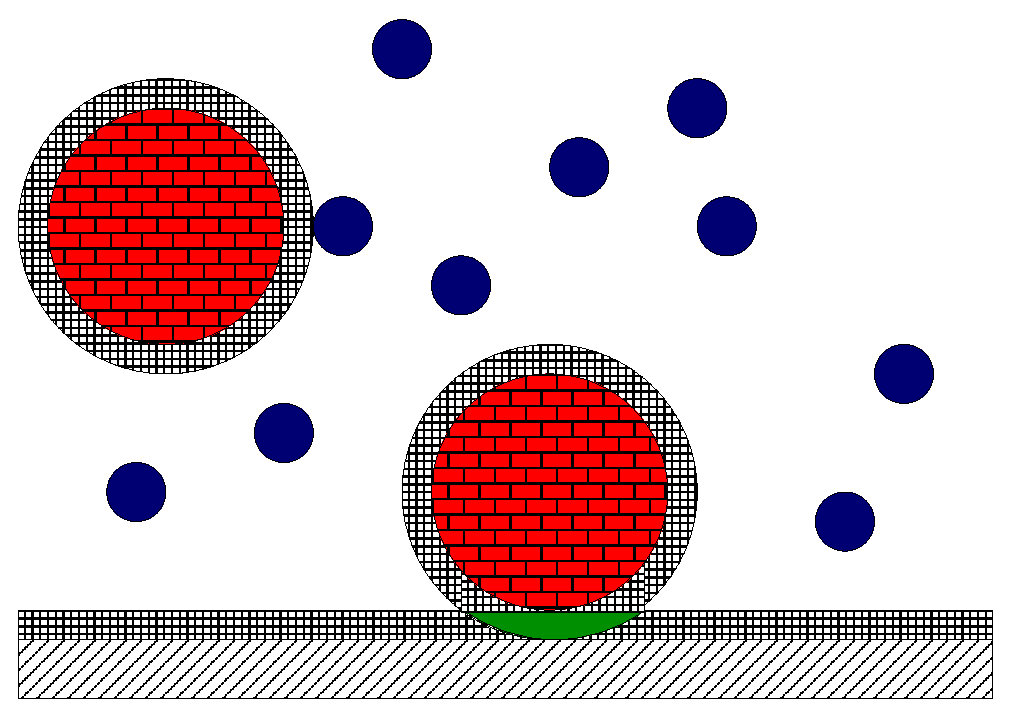
\includegraphics[width=0.7\textwidth]{bilder/kugeln}
   \caption[Gro"se und kleine Harte Kugeln]{Skizze der gro"sen und
     kleinen Kugeln mit "`verbotener Zone"' und deren "Uberlappung}
   \label{abb_skizze_kugeln}
\end{figure}


Wir ziehen um die gro"se Kugel einen Kreis mit Abstand $r$ -- in diesem
Bereich darf sich kein Mittelpunkt einer kleinen Kugel aufhalten (weil
sie hier abgesto"sen w"urde) -- und ebenso um die Wand: Die
"`verbotene Zone"'.  Siehe
Abb. \ref{abb_skizze_kugeln} f"ur eine Skizze.

Um hier die Freie Energie in dem Rein Entropischen System nach
\eqref{eqn_differenz-c3} zu berechnen, ben"otigen wir nur $S$ aus
\eqref{eqn_def_entropie_zustaende} wobei wir $\Omega = V$ verwenden
wollen und $V$ das Volumen angibt, welches die Mittelpunkte der
kleinen Kugeln erreichen k"onnen.\footnote{Wir ignorieren die Entropie,
  die uns die gro"se Kugel mit einbringt, weil es sich ja nur um
  \emph{eine} gro"se handelt, wir aber $N$ kleine (mit $N \gg 1$)
  haben.} F"ur das System gilt:
\begin{equation}
   \label{eqn_differenz-c4}
   \mathcal F = - T \cdot S = - N \cdot K_B \cdot T \cdot \ln V
\end{equation}
Wenn nun die gro"se Kugel nahe an den Rand kommt, "uberschneiden
sich die "`verbotenen Zonen"' von Kugel und Wand und so k"onnen die
kleinen Kugeln effenktiv mehr Raum einnehmen, weil ja ein Teil des
 Volumens quasi doppelt verboten ist\footnote{wobei es f"ur
  die kleinen Kugeln nat"urlich keinen Unterschied macht, ob ein
  Bereich doppelt oder nur einfach verboten ist} und dann entsprechend
dieser Teil an einer anderen Stelle \emph{nicht} verboten ist. 

Unser erreichbares Volumen $V$ vergr"o"sert sich also um $\Delta V$
wobei 
\begin{equation}
   \label{eqn_differenz-c5}
   \Delta V (h) = \frac{1}{3} \cdot \pi \cdot (2r - h)^2 \cdot (3R + r
   + h)
\end{equation}
in Abh"angigkeit vom Abstand $h$ zwischen Kugel(oberfl"ache) und Wand
gegeben ist.\footnote{Diese Formel erh"alt man, wenn man das Volumen
  der Kugelkappe berechnet, die doppelt verboten ist; Siehe
  \textsc{Bronstein}\textsuperscript{7} Kap. 3.3.4}

In Abh"angigkeit von $h$ erhalten wir nun f"ur die "Anderung der Freien
Energie:
\begin{equation}
   \label{eqn_differenz-c6}
   \Delta \mathcal F(h) = -N \cdot K_B \cdot T \cdot \ln \frac{V + \Delta V}{V}
\end{equation}

Damit also $\mathcal F$ minimal wird, muss $\Delta \mathcal{F}$
maximal negativ werden und das erreicht man durch ein m"oglichst gro"ses
$\Delta V$ und damit ein m"oglichst kleines $h$. Wenn also rein
energetisch $h$ sich minimieren soll, bedeutet das, dass die Kugel
sich am Rand aufh"alt. 

\begin{Wichtig}
   Es resultiert also effektiv eine \emph{attraktive} Kraft in
   Richtung Wand, obwohl im System nur repulsive Kr"afte herrschen.
\end{Wichtig}
Interessant ist auch, dass diese Kraft eine \emph{geordnete} Kraft
ist, obwohl die Teilchenst"o"se allesamt ungeordnet sind.





\subsection{Eigenschaften Entropischer Kr"afte}
\label{kap_eigenschaften-entropischer-krafte}

Wir haben gesehen, dass f"ur die entropischen Kr"afte in
Kap. \ref{kap_kristallisation-von-harten-kugeln} gilt:
\begin{itemize}
\item attraktiv (Achtung: In Realit"at gibt es durchaus auch repulsive!)
\item Reichweite: $2r$
\item St"arke: $F \sim \frac{N}{V}$
\end{itemize}

Je nach Form von gro"sen Kugeln und dem Volumen, welches sie insgesamt
einnehmen k"onnen, wird die spontane Kristallisation an verschiedenen
Punkten beginnen (bzw. stattfinden): Die Kugeln werden sich stets so
an der Wand anlagern, dass der "Uberlapp (also die doppelt verbotene
Zone) maximal wird. Siehe dazu Abb. \ref{abb_harte-kugeln_gefaesse}.

Es ist auch m"oglich, statt nur einer gro"sen, mehrere gro"se Kugeln zu
verwenden. Auch hier sorgt die Entropie nach dem selben Schema wieder
daf"ur, dass zwischen den Kugeln eine Anziehung entsteht.

\begin{figure}
   \centering 
   \subfigure{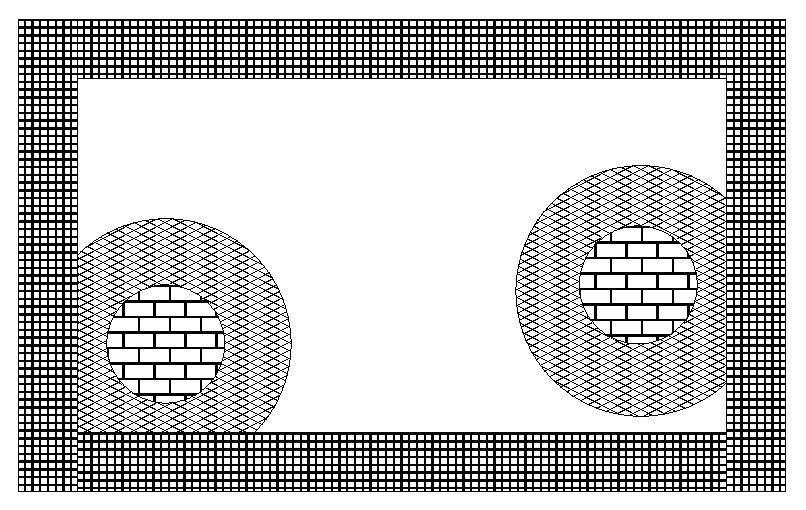
\includegraphics[width=0.45\textwidth]{bilder/kugel_rechteck}}
   \subfigure{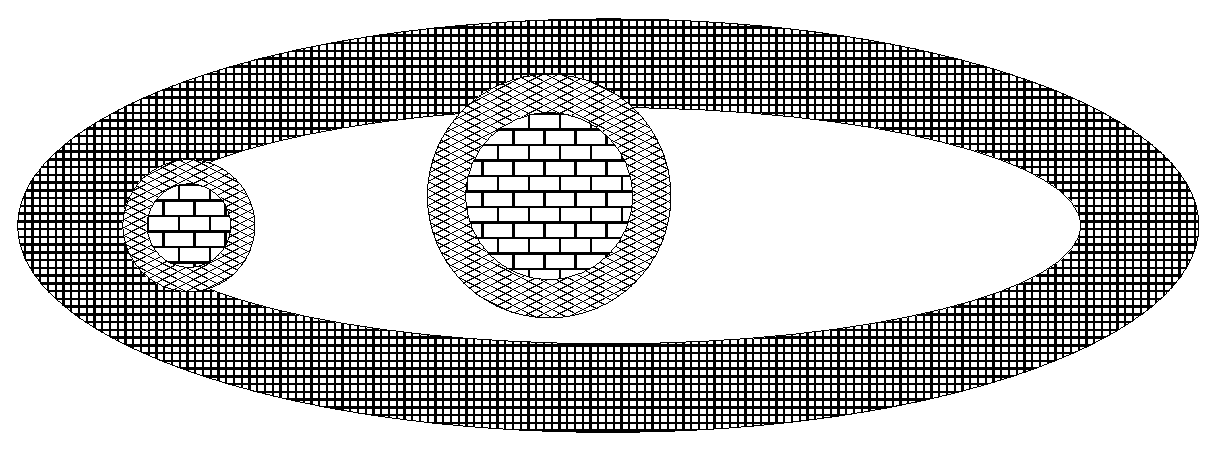
\includegraphics[width=0.45\textwidth]{bilder/kugeln_oval}}
   \caption{Harte Kugeln in verschieden geformten Gef"a"sen}%
   \label{abb_harte-kugeln_gefaesse}
\end{figure}



























%%%%%%%%%%%%%%%%%%%%%%%%%%%%%%%%%%%%%%%%%%%%%%%%%%%%%%%%%%%%%%%%%%%%%%

%%%%%%%%%%%%%%%%%%%%%%%%%%%%%%%%%%%%%%%%%%%%%%%%%%%%%%%%%%%%%%%%%%%%%%

%%%%%%%%%%%%%%%%%%%%%%%%%%%%%%%%%%%%%%%%%%%%%%%%%%%%%%%%%%%%%%%%%%%%%%



